\documentclass[twocolumn, 9pt]{extarticle}
\usepackage{amsmath}
\usepackage{lineno,hyperref}
\usepackage[table,x11names,dvipsnames,table]{xcolor}
\usepackage{authblk}
\usepackage{subcaption,booktabs}
\usepackage{graphicx}
\usepackage{multirow}
\usepackage[nolist,nohyperlinks]{acronym}
\usepackage[superscript]{cite}
\usepackage{tabularx}
\usepackage{cleveref}
\usepackage{float}
\usepackage[group-separator={,}]{siunitx}
\usepackage{geometry}
 \geometry{
 a4paper,
 papersize={210mm,279mm},
 left=12.73mm,
 top=20.3mm,
 marginpar=3.53mm,
 textheight=238.4mm,
 right=12.73mm,
}

\setlength{\columnsep}{6.54mm}

%\linenumbers %%% Turn on line numbers here

\renewcommand{\familydefault}{\sfdefault}

\captionsetup[figure]{labelfont=bf,textfont=normalfont}
\captionsetup[subfigure]{labelfont=bf,textfont=normalfont}


%%%% comment out the below for the other title option
\makeatletter
\def\@maketitle{
\raggedright
\newpage
  \noindent
  \vspace{0cm}
  \let \footnote \thanks
    {\hskip -0.4em \huge \textbf{{\@title}} \par}
    \vskip 1.5em
    {\large
      \lineskip .5em
      \begin{tabular}[t]{l}
      \raggedright
        \@author
      \end{tabular}\par}
    \vskip 1em
  \par
  \vskip 1.5em
  }
\makeatother





\begin{document}


\title{GUSTO Analysis}

\author{Matthew Lyon}

\setcounter{Maxaffil}{0}
\renewcommand\Affilfont{\itshape\small}

\date{}
\maketitle

\section{Introduction}

This is a report on the analysis of the GUSTO data.

\section{Initial Model Development}

These experiments use only a small subset of CpG sites as a pilot study. Specifically, only 383 CpG sites are used within these experiments. Each subject has 4 time points: 3 months, 9 months, 42 months, and 72 months. In this setting, the 3, 9, and 42 months are used to predict the 72nd month. The data are split into training, validation, and test sets with a 80/10/10 split.

\subsection{Time-series Autoencoder}

This set of experiments uses an autoencoder structure, which consists of a CNN encoder, an LSTM layer, and a CNN decoder. The encoder and decoder use 1D convolutions across the feature (CpG site) space, and treat each timepoint independently. As information is passed through the encoder, the feature dimension is reduced. The LSTM layer then processes the reduced feature space across time. Finally, the decoder expands the feature space back to the original dimension. A learned time embedding is added to the input and output of the LSTM to encode the time (in months) into the data. The model had 240K trainable parameters, and the exact number of layers and hyperparameters are detailed in the code, specifically within \texttt{AutoEncoder} class within \texttt{gusto/experiments/cnn\_autoencoder/lib/autoencoder.py}.

\subsubsection{Experiments}
Below are the experiments that were run. The code for each experiment is located in the \texttt{gusto/experiments/cnn\_autoencoder} directory. The models are trained using an $\ell_{1}$ loss function, and results are reported in terms of the root mean squared error (RMSE) on the validation set. the optimiser AdamW is used with a learning rate of $0.001$. The training and validation losses for experiments 1, 2, and 3 are shown in \Cref{fig:losses}.

\paragraph{Experiment 1} The first experiment trains and validates the aforementioned model. The code for this experiment is located in \texttt{experiment\_1.py}. The experiments that follow are modifications of this experiment.

\paragraph{Experiment 2} This experiment uses the same model as Experiment 1, but applies a weighting to the input timepoints as a function of the distance (in time) from the target timepoint. The code for this experiment is located in \texttt{experiment\_2.py}. This modification did not improve the performance of the model.

\paragraph{Experiment 3} This experiment uses the same model as Experiment 1, but interpolates the time dimension of the data. This is done by using a continuously differentiable sub-spline built from piecewise cubic polynomials, known as Akima splines, and implemented in \href{https://docs.scipy.org/doc/scipy/reference/generated/scipy.interpolate.Akima1DInterpolator.html\#scipy.interpolate.Akima1DInterpolator}{scipy}. The data are then resampled using a perturbation in the time dimension of the original 3, 9, and 42 month timepoints. The perturbation is drawn from a Gaussian distribution with a mean of 0 and a standard deviation of 3 months. The code for this experiment is located in \texttt{experiment\_3.py}. The rationale behind this was to allow the model to learn a more continuous representation of the time dimension. This modification did not improve the performance of the model.

\begin{figure}
  \centering
  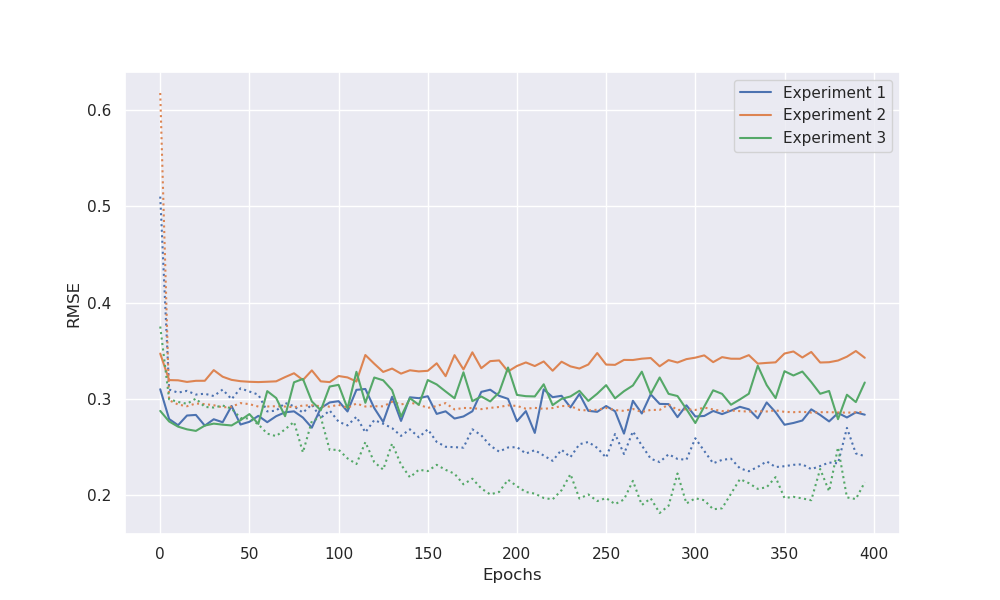
\includegraphics[width=\columnwidth]{plot_experiments_1_to_3.png}
  \caption{Training and validation losses for experiments 1, 2, and 3. Dotted lines indicate the training loss, and solid lines indicate the validation loss.}
  \label{fig:losses}
\end{figure}

\paragraph{Experiment 4} This experiment consisted of a hyperparameter search over the number of layers, kernel sizes, latent dimension size, and use of batch normalisation, within the previous three experiments. Code for this experiment is located in \texttt{experiment\_4.py}. The best hyperparameters, as determined by the validation loss, for each of the three experiments were then used to train a model on the full dataset. The training and validation losses for each of the three experiments are shown in \Cref{fig:losses_hparams}. Overall, the hyperparameter search for each experiment did not yield a significant improvement in the model performance.

\begin{figure}
  \centering
  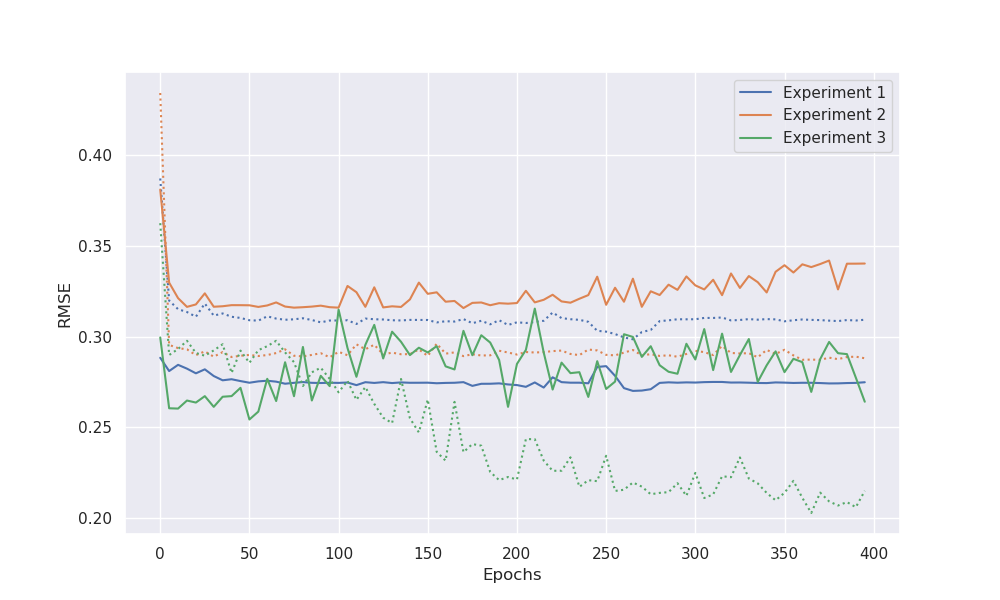
\includegraphics[width=\columnwidth]{plot_experiments_4.png}
  \caption{Training and validation losses for experiments 1, 2, and 3 with hyperparameters determined via hyperparameter search. Dotted lines indicate the training loss, and solid lines indicate the validation loss.}
  \label{fig:losses_hparams}
\end{figure}

\subsection{Independent CpG Sites}

\subsection{Dictionary Learning}

\bibliographystyle{vancouver}
\bibliography{sample}



\end{document}